% Worksheet W2 – Research and writing guide (2 pages)
% Übersetzen: latexmk -xelatex ws-w2-research-and-writing.tex
% ============================================================
% ab-vorlage.tex – gemeinsame Vorlage der Arbeitsblätter
% englisch/12/w-seminar-time/arbeitsblaetter/  (W-Seminar "Time")
% Übersetzen mit:  latexmk -xelatex <datei>.tex   (oder zweimal xelatex)
% Gestaltung wie englisch/13/questions-on-the-text/arbeitsblaetter/ab-vorlage.tex,
% Antwortplatz-Makros (8-mm-Linien) wie informatik/10/java/arbeitsblaetter/ab-vorlage.tex
% Schriften: Carlito (Fließtext), Poppins (Überschriften)
% ============================================================
\documentclass[10pt,a4paper]{article}
\usepackage[a4paper,top=12mm,bottom=13mm,left=14mm,right=14mm,headsep=4mm,headheight=12pt,footskip=7mm]{geometry}
\usepackage{fontspec}
\setmainfont{Carlito}
\newfontfamily\headfont{Poppins}[UprightFont=* Medium, BoldFont=* Medium]
\newfontfamily\headlight{Poppins Light}
\usepackage{xcolor}
\definecolor{prim}{HTML}{2563EB}
\definecolor{primdark}{HTML}{1E3A8A}
\definecolor{sec}{HTML}{7C3AED}
\definecolor{dusk}{HTML}{171A3F}
\definecolor{brass}{HTML}{D9AB2F}
\definecolor{primtint}{HTML}{EFF6FF}
\definecolor{sectint}{HTML}{F5F3FF}
\definecolor{ink}{HTML}{1E293B}
\definecolor{muted}{HTML}{64748B}
\definecolor{rule}{HTML}{CBD5E1}
\definecolor{good}{HTML}{059669}
\definecolor{goodtint}{HTML}{ECFDF5}
\definecolor{warn}{HTML}{B45309}
\definecolor{warntint}{HTML}{FFFBEB}
\definecolor{bad}{HTML}{B91C1C}
\definecolor{badtint}{HTML}{FEF2F2}
% Farben der Zeit-Dimensionen (wie auf der Website)
\definecolor{dlit}{HTML}{B83280}
\definecolor{dphys}{HTML}{2563EB}
\definecolor{dcs}{HTML}{0F8F84}
\definecolor{dpsy}{HTML}{C26A06}
\definecolor{dlang}{HTML}{7C3AED}
\definecolor{dbey}{HTML}{4B5563}
\color{ink}
\usepackage[most]{tcolorbox}
\usepackage{tikz}
\usetikzlibrary{positioning,calc,arrows.meta,shapes.misc}
\usepackage{enumitem}
\setlist{nosep,leftmargin=1.1em,topsep=1pt}
\setlist[itemize]{label=\textcolor{prim}{\small\textbullet}}
\usepackage{tabularx,array,booktabs,colortbl}
\usepackage{multicol}
\usepackage{fancyhdr}
\usepackage{lastpage}
\usepackage{amssymb}
\usepackage{qrcode}
\usepackage{microtype}
\setlength{\parindent}{0pt}
\setlength{\parskip}{0pt}
\linespread{1.02}

% ---------- Kopf- und Fußzeile ----------
\newcommand{\wskopf}{W-Seminar English · Time · Year 12}
\pagestyle{fancy}
\fancyhf{}
\renewcommand{\headrulewidth}{0pt}
\fancyhead[L]{\footnotesize\headlight\textcolor{muted}{\wskopf}}
\fancyhead[R]{\ifnum\value{page}=1\footnotesize\headlight\textcolor{muted}{Name: \rule{38mm}{0.3pt}\quad Date: \rule{18mm}{0.3pt}}\fi}
\fancyfoot[L]{\scriptsize\textcolor{muted}{edu-mrh.de/englisch/12/w-seminar-time}}
\fancyfoot[R]{\scriptsize\textcolor{muted}{\thepage\,/\,\pageref*{LastPage}}}

% ---------- Titel ----------
% \wstitel{Kürzel}{Titel}{Untertitel}
\newcommand{\wstitel}[3]{%
  \begin{tcolorbox}[enhanced,colback=dusk,colframe=dusk,arc=2mm,boxrule=0pt,
     left=4mm,right=4mm,top=2.2mm,bottom=2.2mm,
     interior style={left color=dusk,right color=primdark}]
    \color{white}{\headlight\footnotesize #1}\\[0.3mm]
    {\headfont\LARGE #2}\\[0.6mm]
    {\small #3}
  \end{tcolorbox}\vspace{1mm}}

% ---------- Boxen ----------
% \begin{wsbox}[Optionen]{Nummer}{Überschrift} ... \end{wsbox}
\newtcolorbox{wsbox}[3][]{enhanced,breakable,colback=white,colframe=rule,boxrule=0.5pt,arc=1.5mm,
  left=2.5mm,right=2.5mm,top=1.3mm,bottom=1.3mm,
  title={\headfont\normalsize\textcolor{white}{\colorbox{prim}{\,#2\,}}\;\textcolor{ink}{#3}},
  coltitle=ink,colbacktitle=white,attach title to upper={\par\vspace{0.6mm}},before skip=1.4mm,after skip=1.4mm,#1}
\newtcolorbox{tintbox}[1][]{enhanced,colback=primtint,colframe=primtint,boxrule=0pt,arc=1.2mm,
  left=2mm,right=2mm,top=1.2mm,bottom=1.2mm,#1}
\newtcolorbox{secbox}[1][]{enhanced,colback=sectint,colframe=sectint,boxrule=0pt,arc=1.2mm,
  left=2mm,right=2mm,top=1.2mm,bottom=1.2mm,#1}
\newtcolorbox{goodbox}[1][]{enhanced,colback=goodtint,colframe=goodtint,boxrule=0pt,arc=1.2mm,
  left=2mm,right=2mm,top=1.2mm,bottom=1.2mm,#1}
\newtcolorbox{warnbox}[1][]{enhanced,colback=warntint,colframe=warntint,boxrule=0pt,arc=1.2mm,
  left=2mm,right=2mm,top=1.2mm,bottom=1.2mm,#1}
\newtcolorbox{badbox}[1][]{enhanced,colback=badtint,colframe=badtint,boxrule=0pt,arc=1.2mm,
  left=2mm,right=2mm,top=1.2mm,bottom=1.2mm,#1}

\newcommand{\kl}[1]{{\headfont\small\textcolor{prim}{#1}}}      % kleine Zwischenüberschrift
\newcommand{\klsec}[1]{{\headfont\small\textcolor{sec}{#1}}}
\newcommand{\klc}[2]{{\headfont\small\textcolor{#1}{#2}}}       % Zwischenüberschrift in Farbe
\newcommand{\plus}{\textcolor{good}{\textbf{+}}\ }
\newcommand{\minus}{\textcolor{bad}{\textbf{–}}\ }
\newcommand{\pfeil}{\textcolor{prim}{$\rightarrow$}\ }
\newcommand{\cb}{\raisebox{-0.2ex}{\textcolor{muted}{$\square$}}\ }   % Ankreuzkästchen

% ---------- Antwortplatz (8 mm, wie informatik/10/java) ----------
\newif\ifloesung
\ifdefined\mitloesung \loesungtrue \else \loesungfalse \fi
\newcommand{\lsgfarbe}{\color{sec}\itshape}
\newlength{\zeilenabstand}\setlength{\zeilenabstand}{8mm}
\tikzset{schreiblinie/.style={draw=black!45,line width=0.35pt}}
% Lücke: \luecke[Breite] / \lsg[Breite]{Text}
\newcommand{\lsg}[2][45mm]{%
  \makebox[#1][l]{\rlap{\raisebox{-0.6ex}{\rule{#1}{0.4pt}}}\ifloesung{\lsgfarbe\small\,#2}\fi}}
\newcommand{\luecke}[1][45mm]{\lsg[#1]{}}
% Lücke bis Zeilenende
\newcommand{\lsgrest}[1]{\leavevmode\unskip\hspace{1.5mm}\ifloesung\rlap{\raisebox{0.8pt}{\lsgfarbe\,#1}}\fi\leaders\hbox{\rule[-0.6ex]{0.5pt}{0.4pt}}\hfill\null\par}
\newcommand{\restzeile}{\lsgrest{}}
\newcommand{\lueckentext}{\linespread{1.5}\selectfont\raggedright}
\newcommand{\schreibzeile}{\rule[-2.8mm]{0pt}{8mm}}
% Schreiblinien: \linien{n} / \lsglinien{n}{Text}; erste Linie eine volle Zeilenhöhe unter der Frage
\newcommand{\lsglinien}[2]{\par\vspace{0.5mm}\noindent\begin{tikzpicture}
  \path (0,0) (\linewidth-0.4pt,-#1\zeilenabstand-1.5mm);
  \foreach \i in {1,...,#1}{\draw[schreiblinie] (0.2pt,-\i\zeilenabstand) -- (\linewidth-0.2pt,-\i\zeilenabstand);}
  \ifloesung\node[overlay,anchor=north west,inner sep=0pt] at (1mm,-\zeilenabstand+1pt+5mm) {\parbox[t]{\linewidth-2mm}{\lsgfarbe\raggedright\setlength{\baselineskip}{\zeilenabstand}\rule{0pt}{5mm}#2}};\fi
  \end{tikzpicture}\par}
\newcommand{\linien}[1]{\lsglinien{#1}{}}


\begin{document}

\wstitel{Worksheet W2 · W-Seminar “Time”}{Research and writing guide}%
{From a vague interest to a finished paper: sources, citing, thesis, structure, data – and actually getting started.}

% ------------------------------------------------------------------ 1
\begin{wsbox}{1}{Find sources – and judge them}
\begin{minipage}[t]{0.5\linewidth}\vspace{0pt}
\kl{Where to search}
\begin{itemize}[itemsep=0.3mm]
\item \textbf{Library catalogues}: school, city library, \emph{Bayerische Staatsbibliothek} (OPAC)
\item \textbf{Google Scholar}, JSTOR, open-access journals
\item \textbf{Data}: Destatis, Our World in Data, Google Books Ngram Viewer
\item \textbf{Primary texts}: Project Gutenberg (older literature)
\item \textbf{Snowballing}: read the works cited of a good source
\end{itemize}
\vspace{0.6mm}
{\raggedright\kl{Search smarter}\enspace{\small English keywords · \texttt{"exact phrase"} · \texttt{filetype:pdf} · synonyms (\emph{time perception} / \emph{temporal judgement})}\par}
\end{minipage}\hfill
\begin{minipage}[t]{0.47\linewidth}\vspace{0pt}
\kl{The CRAAP test}\par\vspace{0.4mm}
{\small
\renewcommand{\arraystretch}{1.12}
\begin{tabularx}{\linewidth}{@{}>{\bfseries\color{prim}}l X@{}}
C & \textbf{Currency} – how recent? Does it matter for my topic?\\
R & \textbf{Relevance} – does it answer \emph{my} question?\\
A & \textbf{Authority} – who wrote it? Expert, institution?\\
A & \textbf{Accuracy} – evidence, sources, peer review?\\
P & \textbf{Purpose} – inform, sell, persuade?\\
\end{tabularx}}
\par\vspace{0.6mm}
{\small Wikipedia and AI chatbots are good \emph{starting points} – not sources you cite.}
\end{minipage}
\end{wsbox}

% ------------------------------------------------------------------ 2
\begin{wsbox}{2}{Cite in MLA style (9th edition)}
\begin{minipage}[t]{0.36\linewidth}\vspace{0pt}
\kl{In the text}\par\vspace{0.4mm}
Author's surname + page, no comma:\par
{\small … feel longer in memory (Hammond 47).}\par\vspace{0.6mm}
Quote short passages exactly, paraphrase the rest – \textbf{both} need a citation.\par\vspace{0.6mm}
\kl{Tools}\enspace{\small Zotero (free, browser plug-in), MyBib, Citavi, Word ›References‹. Always check the result.}
\end{minipage}\hfill
\begin{minipage}[t]{0.61\linewidth}\vspace{0pt}
\kl{Works Cited – the core elements in this order}\par\vspace{0.4mm}
\begin{tintbox}\small
Author. \emph{Title of Source.} \emph{Title of Container}, Other contributors, Version, Number, Publisher, Publication date, Location.
\end{tintbox}\par\vspace{0.6mm}
{\small\setlength{\parindent}{-4mm}\leftskip=4mm
\textbf{Book}\enspace Hammond, Claudia. \emph{Time Warped: Unlocking the Mysteries of Time Perception}. Canongate, 2012.\par
\textbf{Article}\enspace Núñez, Rafael E., and Eve Sweetser. “With the Future Behind Them: Convergent Evidence from Aymara Language and Gesture in the Crosslinguistic Comparison of Spatial Construals of Time.” \emph{Cognitive Science}, vol.\,30, no.\,3, 2006, pp.\,401–50.\par
\textbf{AI}\enspace “Explain Vierordt's law in two sentences” prompt. \emph{ChatGPT}, version, OpenAI, 12 Mar.\ 2027, chatgpt.com.\par}
\end{minipage}
\end{wsbox}

% ------------------------------------------------------------------ 3
\begin{wsbox}{3}{From topic to thesis}
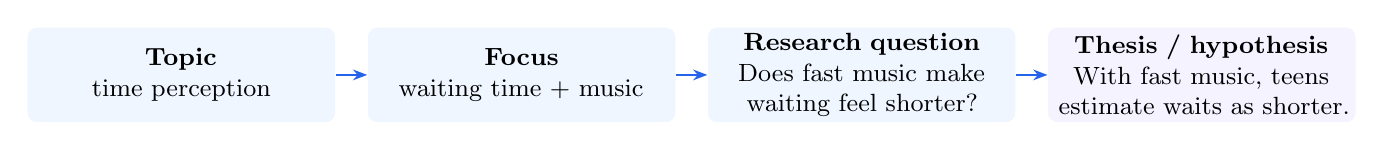
\begin{tikzpicture}[x=1mm,y=1mm,font=\small,
  st/.style={rounded corners=1.2mm,fill=primtint,minimum height=12mm,text width=38mm,align=center,inner sep=1.5pt}]
  \node[st] (a) at (0,0) {\textbf{Topic}\\time perception};
  \node[st,right=4mm of a] (b) {\textbf{Focus}\\waiting time + music};
  \node[st,right=4mm of b] (c) {\textbf{Research question}\\Does fast music make waiting feel shorter?};
  \node[st,right=4mm of c,fill=sectint] (d) {\textbf{Thesis / hypothesis}\\With fast music, teens estimate waits as shorter.};
  \foreach \p/\q in {a/b,b/c,c/d} \draw[-{Stealth[length=1.8mm]},prim,line width=0.8pt] (\p) -- (\q);
\end{tikzpicture}
\par\vspace{1.2mm}
\begin{minipage}[t]{0.5\linewidth}\vspace{0pt}
\kl{A good research question is …}\enspace{\small\textbf{specific} (who, what, where), \textbf{researchable} with your means in a few months, \textbf{open} enough for a real answer, \textbf{relevant} – someone cares about the answer.}
\end{minipage}\hfill
\begin{minipage}[t]{0.47\linewidth}\vspace{0pt}
\minus{\small What is time perception?}\enspace{\footnotesize\textcolor{muted}{(an encyclopaedia entry)}}\par
\plus{\small How does background music change how long Year 12 students think they waited?}
\end{minipage}
\par\vspace{1mm}
\textcolor{sec}{\small\textbf{Your turn:} topic \pfeil focus \pfeil question – first draft, it's allowed to be rough.}
\linien{2}
\end{wsbox}

% ------------------------------------------------------------------ 4
\begin{wsbox}{4}{The structure of your Seminararbeit}
\renewcommand{\arraystretch}{1.18}
\small
\begin{tabularx}{\linewidth}{@{}>{\headfont\color{prim}}l X >{\color{muted}}r@{}}
\arrayrulecolor{rule}
Title page, Abstract & Abstract: 150–200 words – question, method, main result. Write it last. & ½ p.\\
Contents & numbered headings (1, 1.1, 1.2 …) with page numbers & –\\\midrule
1 Introduction & hook, relevance, research question, thesis, how the paper is organised & 1 p.\\
2 Background & key terms, theories and the state of research – \emph{what do others already know?} & 3–4 p.\\
3 Method & your design: material or participants, procedure, measures & 1–2 p.\\
4 Results & tables and charts with short descriptions – no interpretation yet & 2–3 p.\\
5 Discussion & what the results mean, limits of your study, link back to theory & 2–3 p.\\
6 Conclusion & answer to the research question, outlook & 1 p.\\\midrule
Works Cited, Appendix & all sources in MLA style; questionnaire, raw data, AI log, signed declaration & –\\
\end{tabularx}
\end{wsbox}

% ================================================================== page 2
\newpage
% ------------------------------------------------------------------ 5
\begin{wsbox}{5}{Get data you can actually use}
\begin{minipage}[t]{0.485\linewidth}\vspace{0pt}
\klc{dpsy}{Survey}
\begin{itemize}[itemsep=0.3mm]
\item \textbf{Operationalise}: “feels long” \pfeil “How long did you wait? (in minutes)”
\item mostly \textbf{closed questions}, scales from 1 to 5
\item no leading or double questions:\newline
\minus{\small Don't you agree that phones waste time and make us lazy?}
\item \textbf{pilot} with three people, then improve
\item aim for \textbf{30+ answers per group}; anonymous
\end{itemize}
\end{minipage}\hfill
\begin{minipage}[t]{0.485\linewidth}\vspace{0pt}
\klc{dcs}{Experiment}
\begin{itemize}[itemsep=0.3mm]
\item \textbf{one thing you change} (independent variable): music on / off
\item \textbf{one thing you measure} (dependent variable): estimated waiting time
\item \textbf{everything else stays the same}: room, instructions, real waiting time
\item assign people to groups at \textbf{random}
\item write down \emph{exactly} what you did – others must be able to repeat it
\end{itemize}
\end{minipage}
\par\vspace{1mm}
\begin{warnbox}\small\textbf{Before you collect data in school:} ask your teacher – surveys need permission from the school, and under-18s may need parental consent. Never collect names you don't need.\end{warnbox}
\par\vspace{1mm}
\begin{minipage}[t]{0.42\linewidth}\vspace{0pt}
\kl{Make data usable}
\begin{itemize}[itemsep=0.3mm]
\item \textbf{one row} per participant, \textbf{one column} per variable
\item a \textbf{codebook}: what does each column and code mean?
\item clean: incomplete answers out – and say how many
\item \textbf{describe}: n, mean, median, standard deviation
\item \textbf{show}: bar chart or boxplot per group
\item correlation $\neq$ causation!
\end{itemize}
\end{minipage}\hfill
\begin{minipage}[t]{0.55\linewidth}\vspace{0pt}
{\small
\renewcommand{\arraystretch}{1.12}
\begin{tabular}{@{}c c c c@{}}
\arrayrulecolor{rule}\toprule
\textbf{ID} & \textbf{group} & \textbf{age} & \textbf{estimate (s)}\\\midrule
01 & music & 17 & 142\\
02 & silence & 18 & 205\\
03 & music & 17 & 131\\
… & … & … & …\\\bottomrule
\end{tabular}}
\par\vspace{1.2mm}
{\small Spreadsheet functions (English / German Excel):\par
AVERAGE\,/\,MITTELWERT · MEDIAN · STDEV.S\,/\,STABW.S · CORREL\,/\,KORREL}
\end{minipage}
\par\vspace{2mm}
\textcolor{sec}{\small\textbf{Your turn:} What could you measure for your idea – and what would you change?}
\linien{2}
\end{wsbox}

% ------------------------------------------------------------------ 6
\begin{wsbox}{6}{Start writing – before you feel ready}
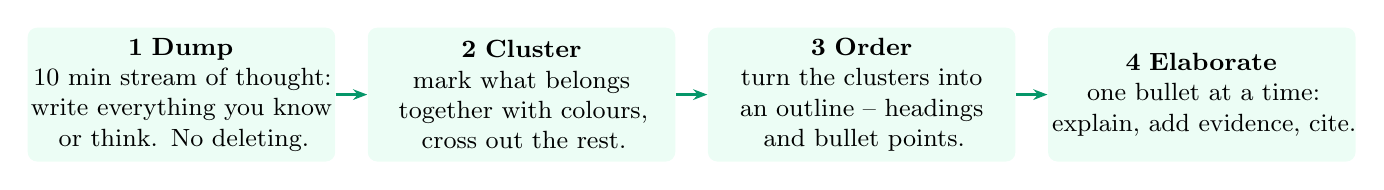
\begin{tikzpicture}[x=1mm,y=1mm,font=\small,
  st/.style={rounded corners=1.2mm,fill=goodtint,minimum height=17mm,text width=38mm,align=center,inner sep=1.5pt}]
  \node[st] (a) at (0,0) {\textbf{1 Dump}\\10 min stream of thought: write everything you know or think. No deleting.};
  \node[st,right=4mm of a] (b) {\textbf{2 Cluster}\\mark what belongs together with colours, cross out the rest.};
  \node[st,right=4mm of b] (c) {\textbf{3 Order}\\turn the clusters into an outline – headings and bullet points.};
  \node[st,right=4mm of c] (d) {\textbf{4 Elaborate}\\one bullet at a time: explain, add evidence, cite.};
  \foreach \p/\q in {a/b,b/c,c/d} \draw[-{Stealth[length=1.8mm]},good,line width=0.8pt] (\p) -- (\q);
\end{tikzpicture}
\par\vspace{1.2mm}
\begin{minipage}[t]{0.5\linewidth}\vspace{0pt}
\begin{itemize}[itemsep=0.4mm]
\item The first draft is \textbf{allowed to be ugly}. Editing is easier than starting.
\item Start where it is easiest – often \textbf{method} or \textbf{results}. Write the introduction last.
\item \textbf{Fixed slot}: same day, same time, every week. 25 minutes on, 5 off.
\item \textbf{Snapshot about every 4 weeks}: hand in your current state, however rough (box 7).
\end{itemize}
\end{minipage}\hfill
\begin{minipage}[t]{0.47\linewidth}\vspace{0pt}
\begin{itemize}[itemsep=0.4mm]
\item End each session with \textbf{one sentence for next time}: “Next: …”
\item Keep your \textbf{research log} and \textbf{AI log} up to date as you go.
\item Stuck? Explain your idea aloud to someone in two minutes – then write down what you said.
\end{itemize}
\par\vspace{1mm}
\kl{My weekly writing slot:}\enspace\luecke[38mm]
\end{minipage}
\end{wsbox}

% ------------------------------------------------------------------ 7
\begin{wsbox}{7}{Plan backwards from the hand-in date: my milestones}
\renewcommand{\arraystretch}{1}
\begin{tabularx}{\linewidth}{@{}>{\raggedright\arraybackslash}p{38mm} X >{\centering\arraybackslash}p{12mm}@{}}
\arrayrulecolor{rule}\toprule
\textbf{by (date)} & \textbf{milestone} & \textbf{done}\\\midrule
\schreibzeile end of 12/1 & topic and first research question fixed & \cb\\\midrule
\schreibzeile every $\sim$4 weeks & snapshot: hand in my current dump / outline / draft & \cb\\\midrule
\schreibzeile & & \cb\\\midrule
\schreibzeile early Nov 2027 & \textbf{hand in the Seminararbeit} & \cb\\\bottomrule
\end{tabularx}
\end{wsbox}

\end{document}
